\chapter{策略型博弈}  \label{c3}

本章我们将系统地讨论非合作博弈论，主题是非合作博弈论中最基本的模型，策略形式的博弈。假设每个参与者可选的行动(称为策略)是已知的，参与者们同时且独立地选择自己的策略，并获得策略组合产生的个体收益，该收益也代表参与者对策略组合的偏好。

如果只有两个参与者，策略形式的博弈可以用一个表格表示，其中一个参与者选择行策略，另一个参与者选择列策略。表格的每个单元格中有对应策略组合下的收益。接下来我们介绍一些标准博弈，如囚徒困境、质量博弈、胆小鬼博弈、性别大战和硬币匹配。

均衡的核心概念是一组相互为最优反应(best response)的策略组合。一个博弈可能有一个、多个或没有均衡。正如第6章所示，纳什(1951)证明了，当引入混合(随机化)策略，每个有限博弈都至少有一个均衡。本章所考虑的无随机化的均衡也被称为纯策略纳什均衡(Nash equilibrium)。

无论其他参与人采取哪种策略，某参与人都严格偏好某一策略而非另一策略，那么称该策略占优另一策略。被占优策略(dominated strategy)在均衡中永远不会被采用，因此可以从博弈中剔除。如果重复剔除劣势策略(iterated elimination of dominated)能够得到唯一的策略组合，那么该博弈被称为占优可解(dominance solvable)博弈。我们用产量竞争的“古诺双寡头博弈(Cournot duopoly)”来说明这一点。(在第4章的4.7节中，我们将把这个博弈转变为一个承诺博弈(commitment game)，即斯塔克尔伯格领导博弈。)

无论其他参与人采取哪种策略，若某一参与者弱偏好某一策略而非另一策略，并且至少在一种博弈结果下严格偏好该策略，那么称该策略弱占优另一策略。剔除一个弱被占优策略(weakly dominated strategy)不会引入新的均衡，但可能会丢失一些均衡，因而不利于全面理解该博弈。除非只希望找到博弈的一个均衡，否则不应该剔除弱被占优策略，更不应该重复这个过程。

3.8节表明，每个参与者有两种策略的(symmetric) \(N\) 人对称博弈总是存在一个均衡。

\section{预备知识和学习目标}

这是本书的第一个核心章节。前一章介绍了拥塞博弈中的策略和均衡概念，前一章有助于理解本章，但它并不是学习本章的必要前提。我们主要处理有限集合。读者应该熟悉集合 \({S}_{1},\ldots，{S}_{N}\) 的笛卡尔积 \({S}_{1} \times  \cdots  \times  {S}_{N}\)。对于策略集为实数区间的古诺博弈，本章将运用初等微积分进行分析。

学习本章后，你应该
\begin{itemize}
\item 了解策略形式博弈的组成部分:策略、策略组合和收益；

\item 能够写出并正确解释两人博弈的表格；

\item 理解均衡的概念，正确使用该术语，并知道它与策略、部分策略组合和最优反应的关系；

\item 熟悉常见的 \(2 \times  2\) 博弈，如囚徒困境(Prisoner’s Dilemma)或猎鹿博弈(Stag Hunt)，并理解它们的区别；

\item 了解占优和弱占优的区别，以及为什么在完整的均衡分析中可以剔除被占优策略，但不能剔除弱被占优策略；

\item 了解古诺产量博弈，包括策略集为实数区间的情况；

\item 理解两人及多人博弈中的对称性。
\end{itemize}

\section{策略型博弈}

策略型博弈是非合作博弈论的基本模型。博弈有 \(N\) 个参与者， \(N \geq  1\)，并且每个参与者 \(i = 1,\ldots，N\) 都有一个非空的策略集 \({S}_{i}\)。如果每个参与者 \(i\) 从 \({S}_{i}\) 中选择一个策略 \({s}_{i}\)，得到的 \(N\) 元组 \(s = \left( {{s}_{1},\ldots，{s}_{n}}\right)\) 被称为一个策略组合，每个参与者 \(i\) 在每个策略组合 \(s\) 下都有对应的实值收益 \({u}_{i}\left( s\right)\)。  

收益代表了每个参与者的偏好。对于两个策略组合 \(s\) 和 \(\widehat{s}\)，如果 \({u}_{i}\left( s\right)  > {u}_{i}\left( \widehat{s}\right)\)，参与者 \(i\) 对\(s\) 的偏好严格强于 \(\widehat{s}\) ；如果 \({u}_{i}\left( s\right)  = {u}_{i}\left( \widehat{s}\right)\)，参与者认为 \(s\) 和 \(\widehat{s}\) 无差异。如果 \({u}_{i}\left( s\right)  \geq  {u}_{i}\left( \widehat{s}\right)\)，则参与者 \(i\)对\(s\) 的偏好不弱于对 \(\widehat{s}\) 的偏好。 参与者 \(i\) 最大化自己的收益，不关心其他参与者的收益(除了试图预测他们的行动)；参与人对某一结果的任何社会性偏好，都必须纳入其自身的收益函数之中，而事实上也都可以通过收益函数加以体现。所有参与者都知道其他参与者可采取的策略和收益，也知道其他参与人同样掌握这些信息，以此类推(该博弈的相关信息是“共同知识”)。

博弈的进行方式如下：所有参与者同时选择自己的策略(不知道其他参与者的选择)，并根据最终形成的策略组合获得各自的收益。参与人之间不能就应当选择何种策略达成任何具有约束力的协议，这也正是此类博弈被称为“非合作博弈”的原因。此外，假设该博弈只进行一次，因此也被称为单次博弈。多次进行相同的博弈(或不同的博弈)会引出更为高深的重复博弈理论。



本书大部分内容讨论两人博弈。参与者通常被命名为$ 1 $和$ 2 $或$ I $和$ II$。策略形式可以用一个表格来表示。表格的行代表参与者$ I$(也称为行参与者)的策略，列代表参与者$ II$(列参与者)的策略。一个策略组合是一个策略对，即一行和一列。表格中对应的单元格包含两个收益，一个是参与者$ I $的，另一个是参与者$ II $的。

如果 \(m\) 和 \(n\) 是正整数，那么一个 \(m \times  n\) 博弈是一个策略形式的两人博弈，参与者 I 有 \(m\) 个策略(表格的行)，参与者 II 有 \(n\) 个策略(表格的列)。

许多重要的博弈论现象在 \(2 \times  2\) 博弈中就已经可以观察到。图~\ref{fig:3.1}(a) 展示了著名的囚徒困境博弈。每个参与者有两个策略，分别称为 \(C\) 和 \(D\)，分别代表“合作”和“背叛”。收益情况如下:如果两个参与者都选择 \(C\)，则两人都获得收益 2。如果两个参与者都选择 \(D\)，则两人都获得收益 1。如果两个参与者选择不同的策略，那么选择 \(C\) 的参与者获得收益 0，选择 \(D\) 的参与者获得最高的收益 3。

\begin{figure}[H]
    \centering
    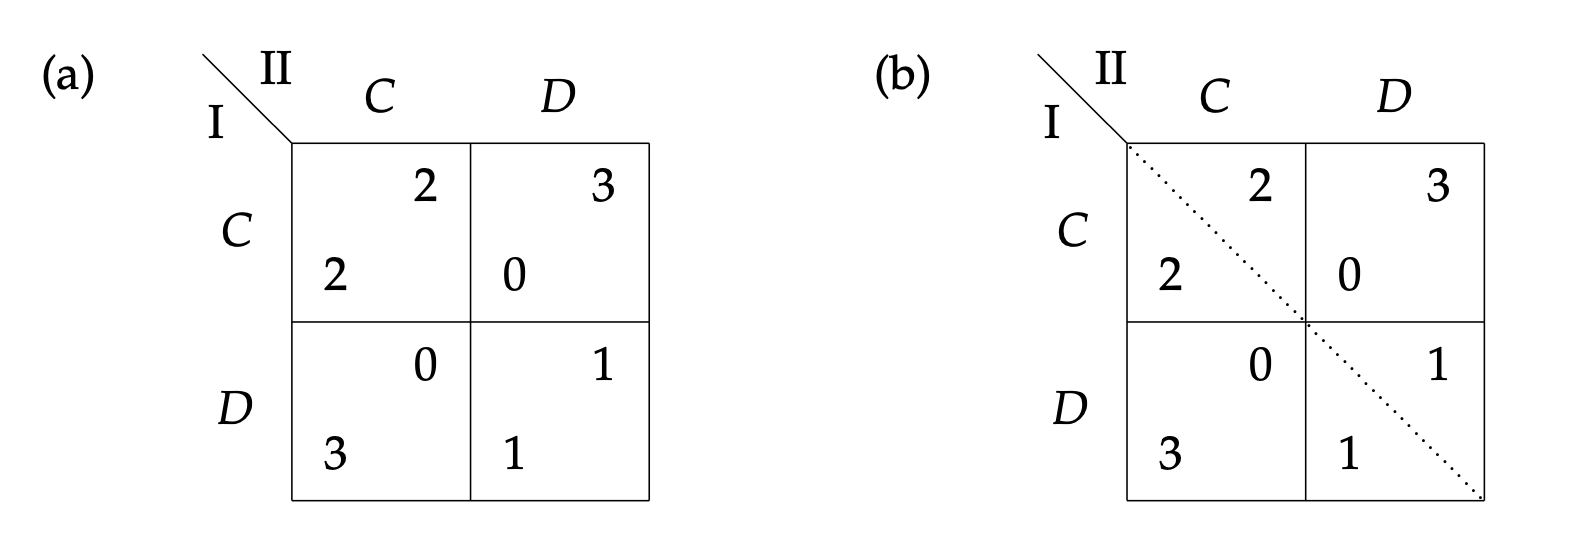
\includegraphics[width=0.8\linewidth]{translation/images/ch03-fig01.png}
    \caption{囚徒困境博弈 (a)，其对称性在 (b) 中通过沿虚线对角线反射显示。}
    \label{fig:3.1}
\end{figure}


在收益表的每个单元格中，行参与者的收益显示在左下角，列参与者的收益显示在右上角。采用这种表示方式有以下几个优点:

\begin{itemize}
\item 收益归属明确。靠近左边的收益靠近行的策略标签，靠近顶部的收益靠近列的标签；这种划分也在表格的左上角显示，那里显示了两个参与者的名称，这里是 I 和 II。

\item 通过沿对角线反射表格(交换参与者、他们的策略(行和列)以及每个单元格中的收益)，可以立即看出该博弈是否是对称的(即，交换参与者后博弈保持不变)，如图~\ref{fig:3.1}(b) 所示。这种反射可行是因为行是从上到下列出的，列是从左到右列出的。

\item 一个 \(m \times  n\) 博弈由两个 \(m \times  n\) 矩阵 \(A\) 和 \(B\) 确定，它们分别包含参与者 I 和参与者 II 的收益。由于每个单元格中的收益是错开的，这两个矩阵很容易分别识别，这样就可以专注于单个参与者的收益。
\end{itemize}

将行参与者的收益置于单元格左下角唯一不常见的方面在于，它位于列参与者的收益下方，而我们通常的惯例是先考虑行，再考虑列。然而，上述原因并不受这一惯例影响，而是对称地(symmetric)对待行和列。另一种采用“先考虑行，再考虑列”这一惯例的常见显示方式(通常出于排版原因)是

\begin{equation}\label{eq:3.1}
\vcenter{\hbox{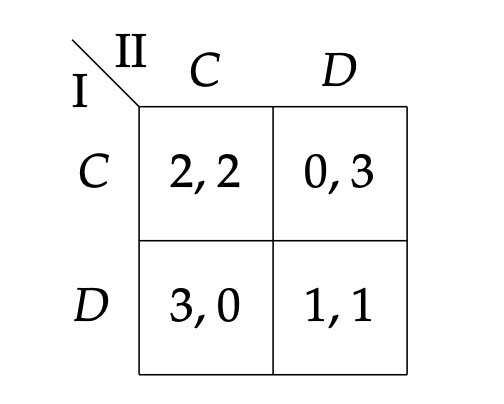
\includegraphics[width=0.3\textwidth]{translation/images/ch03-fig02.png}}}
\end{equation}

在这种显示方式中，收益没有错开，因此更难区分，而且博弈的对称性也不太明显。我们将始终使用如图\ref{fig:3.1}所示的错开收益显示方式。


“囚徒困境”背后的故事涉及两名因涉嫌严重犯罪而被关押的囚犯。除了其中一名囚犯指证另一名囚犯之外，没有其他司法证据证明他们的罪行。如果其中只有一人指证(选择“ \(D\) ”)，他将获得免于起诉的奖励(收益为3)，而另一人将面临长期监禁(收益为0)。如果两人都指证，他们的刑罚都会较轻(每人收益为1)。如果他们均通过完全不指证而相互“合作”(选择“ \(C\) ”)，他们只会因一些可指控的轻微罪行而被短期监禁(每人收益为2)。相对于这种对双方都有利的结果，“背叛”意味着选择指证对方，无论另一名囚犯怎么做，指证都会带来更高的收益。然而，最终两人的收益在相互指证下都会降低。这就构成了他们的“困境”。

在囚徒困境中，两名参与者总是有背叛的动机，因此策略组合(D，D)将是这场博弈的预期结果，尽管如果他们选择(C，C)，两名参与者的情况都会更好。原因在于，非合作博弈模型假定参与人无法强制执行一项共同选择 ((C,C)) 的协议。如果他们能够通过签订某种合同等方式执行这一协议，那么这种做法就必须作为博弈中的一个独立策略加以考虑。囚徒困境表明个人动机可能会损害公共利益。例如，在两个国家的军备竞赛中， \(C\) 和 \(D\) 可能代表限制军备建设和无限制军备建设之间的选择。囚徒困境也可以扩展到多个参与者。例如，通过引入限制每个渔民捕捞量的捕捞配额，不进行过度捕捞以避免鱼类资源减少可能符合每个渔民的利益。如果集体采纳这一措施，将对所有人都有益。然而，如果不执行捕捞配额，每个超过配额的渔民对过度捕捞的影响微乎其微，但自己却能获得巨大利益。从总体上看，他们这样做会破坏鱼类资源。这也被称为“公地悲剧”。这同样适用于许多对环境(以及每个参与者)造成集体损害但对个人有益的行为。

\section{最优反应与均衡}

\begin{figure}
    \centering
    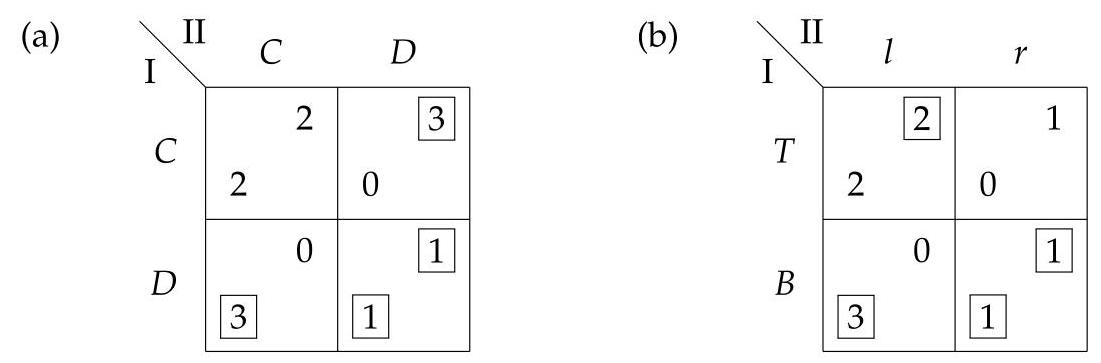
\includegraphics[width=0.8\linewidth]{translation/images/ch03-fig03.jpg}
    \caption{囚徒困境(a)，其中最优反应收益用方框表示，产品质量博弈(b)也是如此。}
    \label{fig:3.2}
\end{figure}

考虑图\ref{fig:3.2}(a)中的囚徒困境，只是添加了更多图形信息以帮助分析该博弈。具体来说，某些收益被方框包围，表明它们是最优反应收益。

最优反应是指在已知其他所有参与者的行动的情况下，对某个参与者而言最优的策略。在两人博弈中，每位参与人只有一个对手。因此，对于行参与人来说，需要针对列参与人的每一个策略分别确定其最优反应。在囚徒困境博弈中，当列参与人选择 \(C\)时，行参与人的最优反应是选择行策略 \(D\)，因为选择\(D\)所获得的收益为$3$，高于选择\(C\)时的收益$2$。因此，在行\(D\)、列\(C\)所对应的单元格中，参与人I的收益$3$被方框标出。当列参与人选择\(D\)时，行参与人的最优反应仍然是选择\(D\)，此时其收益为$1$，同样被方框标出，因为它高于选择行策略\(C\)时的收益$0$。
类似地，当行参与人选择\(C\)时，列参与人的最优反应是选择列策略\(D\)；当行参与人选择\(D\)时，列参与人的最优反应仍然是选择\(D\)。列参与人的这些最优反应收益也由方框标出。由于该博弈是对称的，最优反应收益的分布同样具有对称性。

图\ref{fig:3.2}(b)中的博弈收益与囚徒困境博弈的收益几乎相同，除了右上角单元格中参与者II的收益从3变为1。由于该博弈不是对称的，我们对参与者的策略进行了不同的命名，这里行参与者的策略是 \(T\) 和 \(B\) (分别表示“上”和“下”)，列参与者的策略是 \(l\) 和 \(r\) (分别表示“左”和“右”)。为了更方便地区分它们，我们通常将参与者I的策略用大写字母表示，将参与者II的策略用小写字母表示。


图~\ref{fig:3.2}(b)被称为产品质量博弈。它可以描述参与者I作为餐厅老板的情况，老板可以提供高质量的食物(策略 \(T\) )或低质量的食物(策略 \(B\) )，而潜在客户，即参与者II，可以决定在那里就餐\(l\)或不在那里就餐\(r\)。只有当食物质量好时，客户才会偏好 \(l\) 而非 \(r\)。然而，无论参与者II怎么做，参与者I选择 \(B\) 都会更好。这些偏好通过最优反应框显示出来。参与者II对行 \(T\) 的最优反应与她对行 \(B\) 的最优反应不同。参与者I对任意列的最优反应始终是行 \(B\)。

在图\ref{fig:3.2}的两个博弈中，考虑表格的右下角单元格，在囚徒困境博弈中对应策略组合(D，D)，在产品质量博弈中对应(B，r)。在每个博弈中，这个单元格是唯一两个收益都被框起来的单元格。这意味着定义该单元格的两个策略是相互的最优反应。这样的策略组合被称为均衡，它是非合作博弈的核心解概念。

下面，我们将对一般的\(N\) 人博弈定义最优反应和均衡的概念。

\begin{definition}\label{def:3.1}
    考虑一个具有 \(N\) 个参与者的策略型博弈，其中参与者 \(i = 1,\ldots，N\) 的策略集为 \({S}_{i}\)，并且对于 \({S}_{1} \times  \cdots  \times  {S}_{N}\) 中的每个策略组合 \(s = \left( {{s}_{1},\ldots，{s}_{N}}\right)\)，参与者 \(i = 1,\ldots，N\) 获得收益 \({u}_{i}\left( s\right)\)。对于参与者 \(i\)，考虑其他参与者的部分策略组合
    
    \begin{equation}\label{eq:3.2}
    {s}_{-i} = \left( {{s}_{1},\ldots，{s}_{i - 1},{s}_{i + 1},\ldots,{s}_{N}}\right) 
    \end{equation}
    由其他参与者在 \(j \neq  i\) 时的策略 \({s}_{j}\) 给出。对于 \({S}_{i}\) 中的任何策略 \({s}_{i}\)，这个部分策略组合可以扩展为一个完整的策略组合，记为 \(s = \left( {{s}_{i},{s}_{-i}}\right)\)。那么，如果满足以下条件，则 \({s}_{i}\) 是对 \({s}_{-i}\) 的最优反应

\begin{equation}\label{eq:3.3}
{u}_{i}\left( s\right)  = {u}_{i}\left( {{s}_{i},{s}_{-i}}\right)  \geq  {u}_{i}\left( {{\bar{s}}_{i},{s}_{-i}}\right) \;\text{ 对所有 }{\bar{s}}_{i} \in  {S}_{i}.  
\end{equation}
博弈的一个均衡是一个策略组合 \(s\)，其中每个策略都是对该组合中其他策略的最优反应，即，对于所有参与者 \(i = 1,\ldots，N\)，式(\ref{eq:3.3})都成立。
\end{definition}


除参与者 \(i\) 之外的其他参与者的部分策略组合 \({s}_{-i}\) 的表示法(\ref{eq:3.2})非常常见。对于两人博弈 \(\left( {N = 2}\right)\)，它只是另一个参与者的一个策略。表示法 \(\left( {{s}_{i},{s}_{-i}}\right)\) 为所有参与者创建了一个策略组合 \(s\)，其中假设 \({s}_{i}\) 被插入到第 \(i\) 个位置(作为参与者 \(i\) 的策略)来定义策略组合 \(s\)。条件(\ref{eq:3.3})表明 \({s}_{i}\) 是对 \({s}_{-i}\) 的最优反应，因为参与者 \(i\) 改变成不同的策略 \({\bar{s}}_{i}\)时无法获得更高的收益。收益可能保持不变(在这种情况下， \({\bar{s}}_{i}\) 也是对 \({s}_{-i}\) 的最优反应)。此外，这里只考虑单个参与者的单方面改变，而不考虑多个参与者的联合改变，例如在囚徒困境中从(D，D)变为(C，C)。因此，均衡是一个由互为最优反应的策略构成的策略组合。在这一策略组合中，当其他参与人的策略保持不变时，任何参与人都无法通过单方面改变自己的策略来提高收益。

关于术语的一些说明:均衡通常称为纳什均衡(Nash equilibrium)，以约翰·纳什的名字命名。Nash（1951）证明了对于扩展到包括混合策略的有限策略集(见第6章)，博弈“均衡点”总是存在的。与这种“混合均衡(mixed equilibrium)”不同，根据定义\ref{def:3.1}的均衡通常被称为纯策略均衡(pure equilibrium)，其中参与者确定性地选择他们的策略。

第2章中研究的拥塞博弈是 \(N\) 人博弈，其中每个参与者 \(i\) 的策略集是从其起点 \({o}_{i}\) 到其终点 \({d}_{i}\) 的路径集合，而参与者的收益是其成本的负值，该成本源于使用这条路径上的边的成本，取决于所有参与者对这些边的使用情况。练习~\ref{exer:3.2} 考虑了一个三人博弈，其策略形式由一个合适的“三维”表格直接给出。

为什么均衡是如此重要的概念？对一个博弈的分析，应当说明参与人在遵循自身偏好的情况下将会如何行动，或者应当如何行动，同时还要考虑到其他参与人也会按照自己的偏好行动。
向每位参与人推荐一个策略，就确定了一个策略组合。这个策略组合应当是一个均衡；否则，这一推荐就会自行失效，也就是说，至少有一位参与人有激励偏离被推荐的策略，转而选择另一个策略。
从这个意义上说，对于一个博弈论“解”而言，均衡是其具有“稳定性”的必要条件。这并不意味着均衡总是存在，也不意味着参与人在不断调整策略、使其成为最优反应的过程中总能达到均衡。
在现实中，人们可能并不会按照均衡行动。这可能是因为博弈只是对实际互动情形的一种简化描述；即使博弈具有清晰明确的规则，例如国际象棋，参与人也可能由于问题过于复杂而无法作出完全最优的选择。

本书的许多内容都致力于确定一个博弈的均衡，这是进行博弈论分析的第一步。接下来，还需要另行讨论这些均衡中是否有某些均衡适合作为现实中应当如何行动的建议。分析也可能表明，某个均衡具有不理想的性质，比如在囚徒困境或图\ref{fig:2.3}中的布雷斯悖论中。

\section{多重均衡}

我们考虑几个著名的具有多个均衡的对称博弈。胆小鬼博弈如图\ref{fig:3.3}所示。如虚线所示，该博弈是对称的，方框标记出了最优反应的收益；无论是虚线还是方框，都不是博弈本身描述的一部分，而是对博弈进行分析时添加的标记。两种策略 \(A\) 和 \(C\) 分别代表“激进”和“谨慎”的行为，例如两个司机在狭窄道路上相向行驶的情况。如果另一个参与者采取谨慎策略，激进策略才是有利的(收益为2)，但如果另一个参与者也采取激进策略，就会导致碰撞(收益为0)，而谨慎策略总是给采取该策略的参与者带来收益1。这个博弈有两个均衡，(C, A)和(A, C)，因为对激进行为的最优反应是谨慎，反之亦然。

\begin{figure}
    \centering
    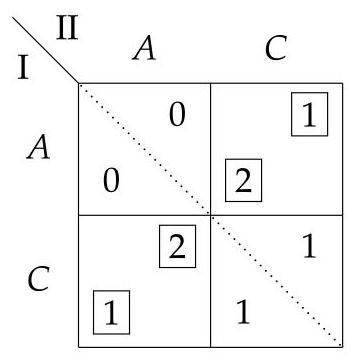
\includegraphics[width=0.3\linewidth]{translation/images/ch03-fig04.jpg}
    \caption{对称的胆小鬼博弈。}
    \label{fig:3.3}
\end{figure}

被称为性别大战的博弈如图\ref{fig:3.4}(a)所示。在这个场景中，参与者I和参与者II是一对情侣，他们各自同时且独立地决定是去听音乐会(C)还是去看体育赛事(S)。参与者从他们去的活动中获得不同的收益，但如果他们独自参加活动，收益就是零。这个博弈有两个均衡：(C, C)，即他们都去听音乐会；或者(S, S)，即他们都去看体育赛事。然而，他们对这些活动的偏好不同。

如图\ref{fig:3.4}(a)所示，性别大战的收益矩阵不是对称的，因为对角线上的策略(C, C)和(S, S)的收益对两个参与者来说并不相同，而这显然是对称的必要条件。然而，改变一个参与者的策略顺序，例如如图\ref{fig:3.4}(b)所示改变参与者I的策略顺序，会使这个博弈具有对称的收益结构；为实现真正的对称博弈，还必须交换参与者I的策略名称 \(C\) 和 \(S\)，但这就不能代表参与者I实际采取的行动了。图\ref{fig:3.4}(b)中的博弈与胆小鬼博弈非常相似。然而，由于策略的含义，性别大战是一个协调博弈(两个参与者都从选择相同的行动中受益)，而胆小鬼博弈是一个“反协调”博弈。

\begin{figure}
    \centering
    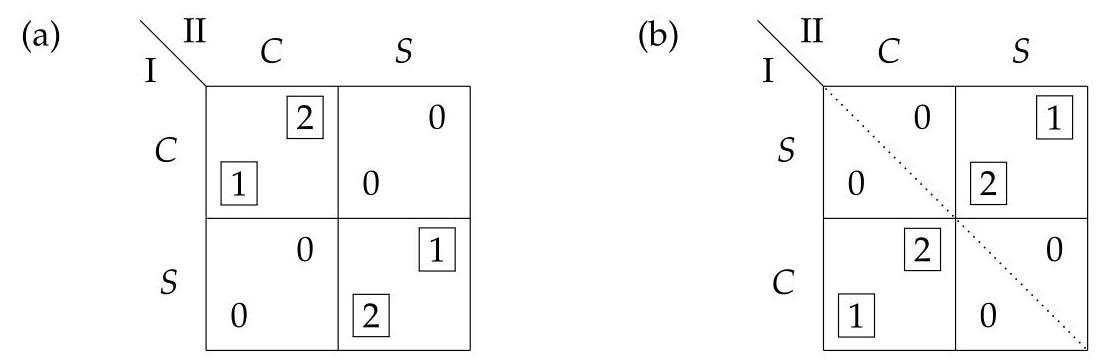
\includegraphics[width=0.8\linewidth]{translation/images/ch03-fig05.jpg}
    \caption{性别大战博弈(a)，如果交换一个参与者的策略，其收益结构就会对称，如图(b)所示。}
    \label{fig:3.4}
\end{figure}


图\ref{fig:3.5}中的猎鹿博弈模型展示了合作与安全之间的冲突。两名猎人各自要在 \(S\) (猎鹿)和 \(H\) (猎兔)之间做出选择。每个猎人无需他人帮助就能捕获野兔，从而获得收益1。要捕获鹿，他们必须合作 - 如果另一个猎人去猎兔，那么猎鹿者的收益为零。如果两人都猎鹿，他们就能成功，且各自获得收益3。

\begin{figure}
    \centering
    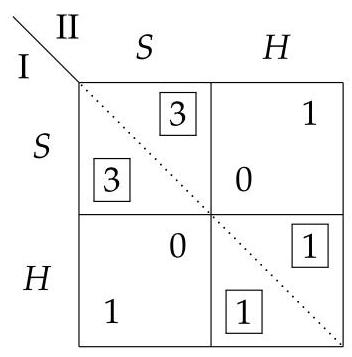
\includegraphics[width=0.3\linewidth]{translation/images/ch03-fig06.jpg}
    \caption{猎鹿博弈}
    \label{fig:3.5}
\end{figure}


这个对称博弈有两个对称均衡，即(S, S)和(H, H)。第一个均衡为双方带来的收益要高得多，但这需要信任对方也会选择 \(S\)，因为无论对方怎么做，选择 \(H\) 都是完全安全的。出于这个原因，猎鹿博弈有时也被称为“信任困境”。

如果博弈论能为如何在多个均衡中进行选择提供指导，那将非常有用。在猎鹿博弈中，推荐选择(S, S)似乎非常合理，因为与选择(H, H)相比，双方的收益都更高，而且如果对方也选择 \(S\)，那么选择 \(S\) 会更好。然而，仅靠这种推理是站不住脚的，因为它同样适用于该博弈的以下变体。假设图\ref{fig:3.5}中每个收益$1$都被替换为$290$万，收益$3$都被替换为$300$万，那么参与者选择 \(S\) 可能获得$300$万美元(但如果对方选择 \(H\)，则有一无所获的风险)，或者选择 \(H\) 安全地获得290万美元。在这里，无风险的选择显然更好。

对于均衡选择问题，存在许多不同的研究方法。通常，人们会要求一个均衡满足某些额外的精炼标准，而这些标准应当具有一般适用性。例如，可以要求不存在另一个能使两位参与人都获得更高收益的均衡。不过，正如猎鹿博弈所表明的那样，这一要求可能与某个均衡本身所具有的“风险性”相冲突。
这些标准能否普遍适用，往往也存在争议，因为它们可能要求参与人运用相同的理论推理过程，才能共同选出所谓“正确的”均衡。本书不打算解决这一问题，而只满足于判断一个博弈何时具有多个均衡。

\section{被占优策略}

在图\ref{fig:3.2}(b)的产品质量博弈中，无论对方参与者选择什么策略，行参与者选择策略 \(B\) 的收益都比选择策略 \(T\) 更高。我们说 \(B\) 严格占优 \(T\)。以下定义阐述了一般 \(N\) 人博弈中严格占优、弱占优和收益等价的概念。

\begin{definition}\label{def:3.2}
    考虑一个 \(N\) 人博弈，每个参与者 \(i = 1,\ldots，N\) 的策略集为 \({S}_{i}\)，收益函数为 \({u}_{i}\)，设 \({s}_{i}\) 和 \({t}_{i}\) 是某个参与者 \(i\) 的两个策略， \({S}_{-i} = \mathop{\sum }\limits_{{j = 1,j \neq  i}}^{N}{S}_{j}\) 是其他参与者的部分策略组合集合。那么

\begin{itemize}
\item 如果满足以下条件，则 \({t}_{i}\) 占优(或严格占优) \({s}_{i}\)

\begin{equation}\label{eq:3.4}
{u}_{i}\left( {{t}_{i},{s}_{-i}}\right)  > {u}_{i}\left( {{s}_{i},{s}_{-i}}\right) \;\forall {s}_{-i} \in  {S}_{-i}, 
\end{equation}

\item 如果满足以下条件，则 \({t}_{i}\) 与 \({s}_{i}\) 收益等价

\[
{u}_{i}\left( {{t}_{i},{s}_{-i}}\right)  = {u}_{i}\left( {{s}_{i},{s}_{-i}}\right) \;\forall {s}_{-i} \in  {S}_{-i},
\]


\item 如果 \({t}_{i}\) 和 \({s}_{i}\) 收益不等价，且满足以下条件，则 \({t}_{i}\) 弱占优 \({s}_{i}\)


\begin{equation}\label{eq:3.5}
{u}_{i}\left( {{t}_{i},{s}_{-i}}\right)  \geq  {u}_{i}\left( {{s}_{i},{s}_{-i}}\right) \;\forall {s}_{-i} \in  {S}_{-i}. 
\end{equation}
\end{itemize}

\end{definition}

在两人博弈中，严格占优的条件(\ref{eq:3.4})特别容易验证。例如，如果 \(i\) 是列参与者，那么 \({s}_{i}\) 和 \({t}_{i}\) 是两列， \({s}_{-i}\) 是任意一行，我们观察列参与者的收益。那么(\ref{eq:3.4})表明，逐行来看，列 \({t}_{i}\) 中的每个元素都大于列 \({s}_{i}\) 中的相应元素。对于图\ref{fig:3.2}(a)中囚徒困境博弈里的列 \(D\) 和 \(C\)，这可以写成 \(\left( \begin{array}{l} 3 \\  1 \end{array}\right)  > \left( \begin{array}{l} 2 \\  0 \end{array}\right)\)，条件(\ref{eq:3.4})成立的。然而，对于图\ref{fig:3.2}(b)中的产品质量博弈， \(r\) 和 \(l\) 的两个收益列分别是 \(\left( \begin{array}{l} 1 \\  1 \end{array}\right)\) 和 \(\left( \begin{array}{l} 2 \\  0 \end{array}\right)\)，条件(\ref{eq:3.4})不成立， \(r\) 既不占优 \(l\)， \(l\) 也不占优 \(r\)。不过，对于这两个博弈(行参与者的收益相同)，底行占优顶行，因为\(\begin{pmatrix}3&1\end{pmatrix} > \begin{pmatrix}2&0\end{pmatrix}\)(我们逐分量比较两个向量)。

请注意，\({t}_{i}\) 占优 \({s}_{i}\)并不意味着 \({t}_{i}\) 总是比 \({s}_{i}\) 更好。在囚徒困境中， \(D\) 占优 \(C\)，但在另一个参与者采用不同策略的情况下，选择 \(D\) 可能得到收益1，选择 \(C\) 可能得到收益2。

弱占优本质上与严格占优相同，只是式((\ref{eq:3.4}))中的严格不等式被式((\ref{eq:3.5}))中的弱不等式所取代，但不能始终取等号(这意味着收益等价)。也就是说，如果式(\ref{eq:3.5})成立，并且对于至少一个部分策略组合 \({s}_{-i} \in  {S}_{-i}\) 有 \({u}_{i}\left( {{t}_{i},{s}_{-i}}\right)  > {u}_{i}\left( {{s}_{i},{s}_{-i}}\right)\)，那么 \({t}_{i}\) 弱占优 \({s}_{i}\)。

\begin{figure}
    \centering
    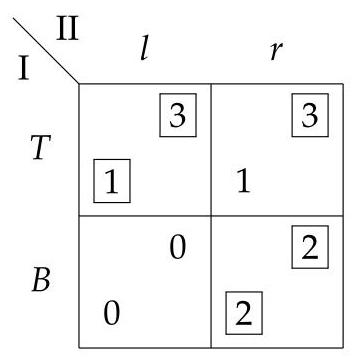
\includegraphics[width=0.3\linewidth]{translation/images/ch03-fig07.jpg}
    \caption{一个列 \(r\) 弱占优列 \(l\) 的博弈。弱被占优策略 \(l\) 是均衡(T，l)的一部分。}
    \label{fig:3.6}
\end{figure}


图\ref{fig:3.6}展示了一个博弈，其中参与者I的策略 \(T\) 有两个最优反应， \(l\) 和 \(r\)，因为它们给参与者II带来相同的收益(实际上给参与者I也带来相同收益，但参与者I不选择列)。对于行 \(B\)，参与者II选择 \(l\) 的收益比选择 \(r\) 的收益差，所以 \(l\) 被 \(r\) 弱占优。然而， \(l\) 是一个均衡，即$(T，l)$的一部分，实际上给参与者II带来的收益比均衡$(B，r)$更高，所以可以说参与者II在“威胁”选择 \(l\) 时具有优势。因此，在分析博弈时，不应该忽视弱被占优策略，因为通常人们感兴趣的是找出博弈的所有均衡。

相比之下，在均衡中，参与者永远不会选择严格被占优策略，因为他可以选择占优该策略的策略。下面的命题考虑了从博弈中移除弱被占优或严格被占优策略时会发生什么。

\begin{proposition}\label{prop:3.3}
    考虑一个策略集为 \({S}_{1},\ldots,{S}_{N}\) 的 \(N\) 人策略形式博弈 \(G\)。设 \({s}_{i}\) 和 \({t}_{i}\) 是参与者 \(i\) 的两个不同策略。假设 \({t}_{i}\) 弱占优于 \({s}_{i}\) 或与 \({s}_{i}\) 收益等价。考虑与 \(G\) 具有相同收益函数，但 \({S}_{i}\) 被 \({S}_{i} - \left\{  {s}_{i}\right\}\) 替代的博弈 \({G}^{\prime }\)。那么:

(a) \({G}^{\prime }\) 的任何均衡都是 \(G\) 的均衡。

(b) 如果 \({t}_{i}\) 占优于 \({s}_{i}\)，那么 \(G\) 和 \({G}^{\prime }\) 具有相同的均衡。

\end{proposition}

\begin{proof}
    为了证明 (a)，考虑 \({G}^{\prime }\) 的一个均衡，它是 \(G\) 中的一个有效策略组合。如果参与者 \(i\) 在 \(G\) 中可以通过偏离到策略 \({s}_{i}\) 获得收益，那么显然，参与者 \(i\) 在 \({G}^{\prime }\) 中也可以通过偏离到 \({t}_{i}\) 获得收益，这违反了均衡性质。除参与者 \(i\) 之外的其他参与者的均衡性质成立，因为他们在 \(G\) 和 \({G}^{\prime }\) 中有相同的策略和收益。

为了证明 (b)，假设 \({t}_{i}\) 占优于 \({s}_{i}\)。根据 (\ref{eq:3.4})，由于参与者 \(i\) 可以通过偏离到 \({t}_{i}\) 获得收益，被占优策略 \({s}_{i}\) 永远不会是均衡 \(s = \left( {{s}_{i},{s}_{-i}}\right)\) 的一部分。 \(G\) 中任何不包含 \({s}_{i}\) 的策略组合也是 \({G}^{\prime }\) 的一个策略组合。如果该组合是 \(G\) 的一个均衡，那么它也是 \({G}^{\prime }\) 的一个均衡，因为 \({G}^{\prime }\) 的偏离可能性更少。根据 (a)， \({G}^{\prime }\) 中的任何均衡也是 \(G\) 中的均衡。因此，\(G\) 和 \({G}^{\prime }\) 具有相同的均衡。
\end{proof}


如之前结合图~\ref{fig:3.6}所解释的，剔除一个弱被占优策略可能会导致博弈的均衡丢失。命题~\ref{prop:3.3}(a)表明这不会引入新的均衡。因此，当试图仅找到博弈的一个均衡时，剔除一个弱被占优策略可以被认为是可接受的。然而，这通常会扭曲对博弈的分析。

命题\ref{prop:3.3}(b)表明，从博弈中剔除一个(严格)被占优策略不会改变其均衡。因为一个追求收益最大化的参与者不应该采用被占优策略，所以从参与者的策略集中剔除被占优策略，从而将其从博弈中消除是有意义的。这会改变博弈，并且更小的博弈可能会有之前未被占优的新的被占优策略。再次剔除这样的被占优策略，并持续这个过程直到所有剩余策略都未被占优，这被称为重复剔除劣势策略。

相比之下，剔除弱被占优策略是有问题的，因为它可能会丢失均衡，并且在重复操作时会引入更多问题。如练习~\ref{exer:3.1} 所示，剔除弱被占优策略的顺序通常是重要的。这个过程可能会陷入停滞，因为弱占优会变成收益等价，除非同时剔除一个收益等价的策略，而关于应该剔除哪个策略的决策相当随意。此外，即使剔除弱被占优策略得到了一个单一的策略组合，该组合也可能依赖于剔除顺序。

图\ref{fig:3.7}展示了产品质量博弈的重复剔除劣势策略过程。第一步，顶行 \(T\) 被 \(B\) 占优并被剔除，形成一个 \(1 \times  2\) 博弈。在那个博弈中，列 \(r\) 占优于 \(l\) (在原始的 \(2 \times  2\) 博弈中并非如此)。剔除 \(l\) 后，剩下一个单元格，对应策略组合 $(B, r)$，它也是原始博弈的唯一均衡。以下命题表明这通常是成立的。

\begin{figure}
    \centering
    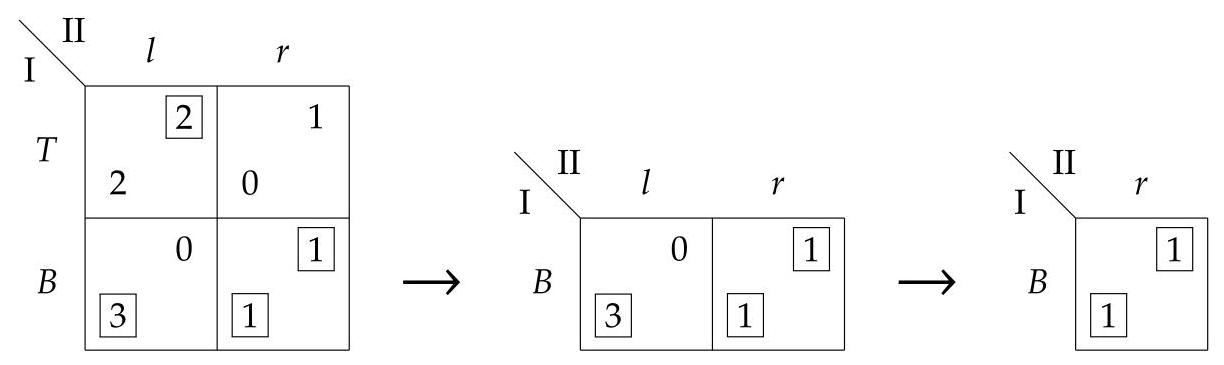
\includegraphics[width=0.8\linewidth]{translation/images/ch03-fig08.jpg}
    \caption{产品质量博弈中的重复剔除劣势策略。}
    \label{fig:3.7}
\end{figure}

\begin{proposition}\label{prop:3.4}
    考虑一个博弈G，通过有限次重复剔除严格被占优策略将其简化为单一的策略组合 \(s\) (即每个参与者只有一种策略)。那么 \(s\) 是 \(G\) 的唯一均衡。
\end{proposition}

\begin{proof}
    根据假设，从 \(G\) 中剔除一个(被占优)策略，并在有限步骤内继续此过程，为每个参与者得到单一策略。最终的博弈只有一个策略组合 \(s\)，这显然是一个均衡，因为没有参与者可以偏离。根据命题~\ref{prop:3.3}，前一个博弈有相同的唯一均衡 \(s\)，通过在生成的博弈序列中逆向推导，这最终对原始博弈 \(G\) 也成立。
\end{proof}

如果有限次重复剔除劣势策略以唯一的策略组合结束，则称该博弈是占优可解的，最终的策略组合即为其解，这也是该博弈的唯一均衡。以下引理表明了一个令人放心的事实，即剔除(被占优)策略的顺序无关紧要，并且可以同时剔除多个(被占优)策略。

\begin{proposition}\label{prop:3.5}
    考虑一个具有策略集 \({S}_{1},\ldots\), \({S}_{N}\) 的 \(N\) 个参与者的策略形式博弈 \(G\)，设 \({s}_{i}\) 和 \({\widehat{s}}_{j}\) 分别是参与者 \(i\) 和参与者 \(j\) 的两个(被占优)策略，可能是同一个参与者 \(\left( {i = j}\right)\)。设 \({G}^{\prime }\) 是从 \(G\) 中通过从 \({S}_{i}\) 移除 \({s}_{i}\) 得到的(其他方面不变)博弈，设 \(\widehat{G}\) 是从 \(G\) 中通过从 \({S}_{j}\) 移除 \({\widehat{s}}_{j}\) 得到的博弈。那么 \({\widehat{s}}_{j}\) 在 \({G}^{\prime }\) 中是(被占优)策略， \({s}_{i}\) 在 \(\widehat{G}\) 中是(被占优)策略，并且从 \({G}^{\prime }\) 移除 \({\widehat{s}}_{j}\) 和从 \(\widehat{G}\) 移除 \({s}_{i}\) 得到的博弈与直接从 \(G\) 移除 \({s}_{i}\) 和 \({\widehat{s}}_{j}\) 得到的博弈相同。
\end{proposition}

\begin{proof}
    假设 \({s}_{i}\) 被 \({t}_{i}\) 占优， \({\widehat{s}}_{j}\) 被 \({\widehat{t}}_{j}\) 占优。如果 \({\widehat{t}}_{j} \neq  {s}_{i}\)，那么 \({\widehat{s}}_{j}\) 在 \({G}^{\prime }\) 中也被 \({\widehat{t}}_{j}\) 占优，因为 \({G}^{\prime }\) 中的任何部分策略组合 \({s}_{-j}\) 也是 \(G\) 中的部分策略组合，在其中占优不等式成立。如果 \({\widehat{t}}_{j} = {s}_{i}\) (这需要 \(i = j\) )，那么 \({\widehat{s}}_{j}\) 在 \({G}^{\prime }\) 中也被 \({t}_{i}\) 占优(因为占优显然是传递的)，如所声称的那样。类似地，如果 \({t}_{i} \neq  {\widehat{s}}_{j}\)，那么 \({s}_{i}\) 在 \(\widehat{G}\) 中被 \({t}_{i}\) 占优，如果 \({t}_{i} = {\widehat{s}}_{j}\)，那么 \({s}_{i}\) 在 \(\widehat{G}\) 中被 \({\widehat{t}}_{j}\) 占优。显然，剔除(被占优)策略会得到与直接从 \(G\) 剔除 \({s}_{i}\) 和 \({\widehat{s}}_{j}\) 相同的博弈。
\end{proof}

重复剔除严格被占优策略有两个用途。首先，它可以简化博弈，理想情况下，直到只剩下一个策略组合，这就是该博弈的唯一均衡(当然，这只有在博弈只有一个均衡时才有效)。其次，选择均衡策略假设其他参与者也会选择他们的均衡策略。然而，无论其他参与者选择什么策略，参与者总是会更喜欢占优策略而不是被占优策略。从这个意义上说，选择占优策略在对其他参与者行为的假设方面更“稳健”。这当然适用于在原博弈中占优的策略；重复剔除劣势策略确实需要“理性”假设，即其他参与者会最大化他们的收益(在图\ref{fig:3.7}中，参与者II假设参与者I不会选择 \(r\) 而选择 \(T\) )。

\section{数量竞争的古诺双寡头模型}

本节讨论一个描述两家企业之间竞争的经济模型，两家企业分别选择各自产品的产量，而市场价格随着市场总产量的增加而下降。该模型由奥古斯丁·古诺（Augustin Cournot）于1838年提出，因此也称为古诺双寡头模型（Cournot duopoly）。在这一博弈中，参与人的策略集是无限集。该博弈的有限版本是占优可解的；原则上，无限版本也可以采用类似的方法求解，我们将在本节末对此加以说明。

参与人I和II代表两家企业，它们分别选择生产某种商品的非负产量，假设产量存在某个上限\(M\)，因此 \({S}_{1} = {S}_{2} = \left\lbrack  {0,M}\right\rbrack\)。设 \(x\) 和 \(y\) 分别是参与人 I 和 II 选择的策略。为简单起见，假设没有生产成本，总产量 \(x + y\) 以每单位 \({12} - \left( {x + y}\right)\) 的价格在市场上出售。由于不存在生产成本，该价格也是企业每单位商品的利润，因此参与人I和II的收益 \(a\left( {x,y}\right)\) 和 \(b\left( {x,y}\right)\)分别为

\begin{equation}\label{eq:3.6}
\begin{aligned}
    &\text{ 参与人I的收益 } : \;a\left( {x,y}\right)  = x \cdot  \left( {{12} - y - x}\right) \text{， } \\
    &\text{ 参与人II的收益 } :   \;b\left( {x,y}\right)  = y \cdot  \left( {{12} - x - y}\right) \text{ . }
\end{aligned}
\end{equation}

\begin{center}
\setlength{\fboxsep}{6pt}
\setlength{\fboxrule}{0.4pt}
\fbox{
    \parbox{\dimexpr\linewidth-2\fboxsep-2\fboxrule\relax}{
        \(\Rightarrow\)\quad 练习~\ref{exer:3.3} 描述了一个包含生产成本的扩展模型。
    }
}
\end{center}

博弈(\ref{eq:3.6})在 \(x\) 和 \(y\) 上是对称的。图\ref{fig:3.8}展示了这个博弈的一个有限版本，其中参与人的策略被限制在四个产量水平上:0 、3、4 或 6。收益由(\ref{eq:3.6})式确定。例如，当 \(x = 3\) 和 \(y = 4\) 时，参与人I的收益为$15$，参与人II的收益为$20$。由这个收益表确定的最优反应收益用方框标出。该博弈有唯一的均衡$(4,4)$，此时每个参与人的收益均为$16$。

\begin{figure}
    \centering
    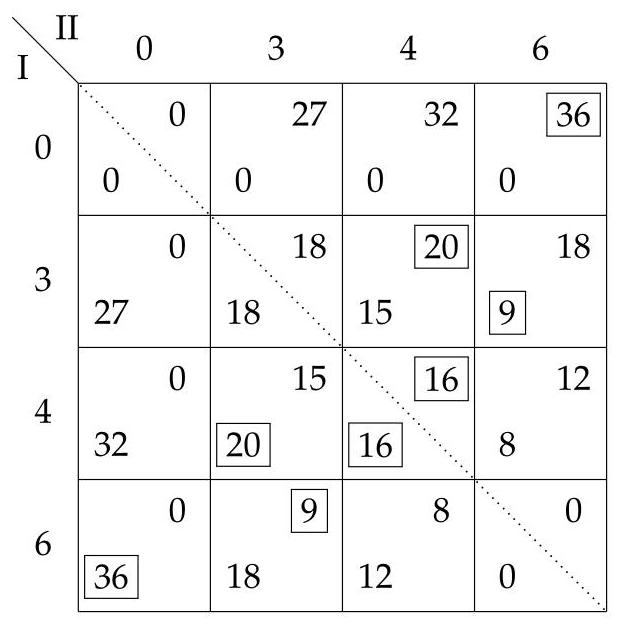
\includegraphics[width=0.4\linewidth]{translation/images/ch03-fig09.jpg}
    \caption{两家企业之间的对称双寡头博弈，两家企业都有四个策略:0、3、4、6，当参与人I选择 \(x\)，参与人II选择 \(y\)。收益由\eqref{eq:3.6}式确定。}
    \label{fig:3.8}
\end{figure}

\begin{figure}
    \centering
    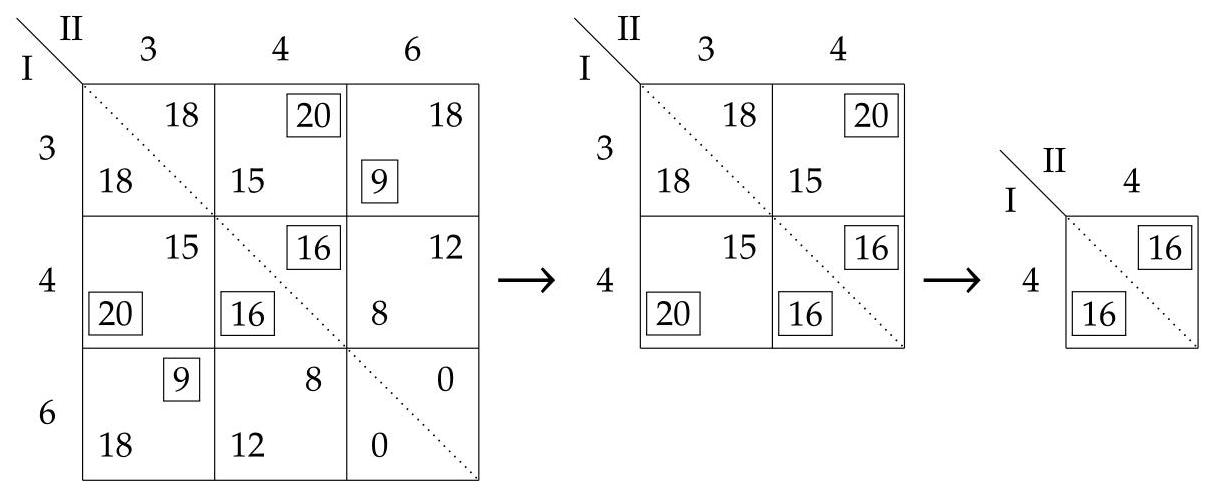
\includegraphics[width=0.8\linewidth]{translation/images/ch03-fig10.jpg}
    \caption{对图~\ref{fig:3.8}中的博弈依次进行占优策略剔除：首先剔除双方的策略 \(0\)，然后剔除被 \(4\) 占优的策略 \(6\)，最后剔除被 \(4\) 占优的策略 \(3\)。由此可见，该博弈是占优可解的。}
    \label{fig:3.9}
\end{figure}

图\ref{fig:3.9}表明，该博弈可以通过重复剔除劣势策略来求解。在最初的\(4 \times  4\) 博弈中，策略 $0$ 被 $3$ 或 $4$ 占优，对两个参与人直接剔除该策略后，得到图\ref{fig:3.9}左侧所示的 \(3 \times  3\) 博弈。在那个博弈中，策略 $6$ 被 $4$ 占优。为两个参与人剔除该策略后，得到中间的 \(2 \times  2\) 博弈。这个博弈具有囚徒困境的结构，因为 $4$ 占优 $3$，因此 $3$ 将被剔除，但最终保留下来的策略组合$(4,4)$给双方带来的收益缺低于策略组合$(3,3)$。这里，囚徒困境出现在经济背景中：两家企业如果能够合作，可以平均分配最优的“垄断”产量 $6$，即各自生产$3$ 单位，但是当一家企业选择产量$3$时，另一家企业会“背叛”并将产量提高到$4$。如果两家企业都这样做，总产量将增加到$8$，市场价格将降至 $4$，两家企业的收益都会降低。

当每个参与人的策略集为实数区间 \(\left\lbrack  {0,M}\right\rbrack\)时，也可以对该博弈进行分析。我们可以假设 \(M = {12}\)，因为如果某个参与人选择的产量高于12，那么价格 \({12} - x - y\) 将为负，此时该参与人会选择不生产。参与人 I 对 \(y\) 的最优反应是使 \(a\left( {x,y}\right)\) 最大化的产量 \(x\)，其中

\begin{equation}\label{eq:3.7}
    a\left( {x,y}\right)  = x \cdot  \left( {{12} - y - x}\right)  =  - {\left( x - \frac{{12} - y}{2}\right) }^{2} + {\left( \frac{{12} - y}{2}\right) }^{2}
\end{equation}

显然，该函数在 \(x = \frac{{12} - y}{2} = 6 - y/2\) 处取得最大值，其中 \(x \geq  0\)，因为 \(y \leq  {12}\)。(仅考虑 \(x \cdot  \left( {{12} - y - x}\right)\) 时，这是一条抛物线，其顶点位于零点 \(x = 0\) 和 \(x = {12} - y\) 的中点。此外，通过求解一阶条件 \(\left. {\frac{d}{dx}a\left( {x,y}\right)  = 0\text{ 也可以得到同样的最大值点。 }}\right)\) 注意，对于每一个给定的 \(y\)，参与人 I 的最优反应都是唯一的。由于该博弈是对称的，参与人 II 对 \(x\) 的最优反应同样是唯一的，并由 \(y = 6 - x/2\) 给出。

\begin{figure}
    \centering
    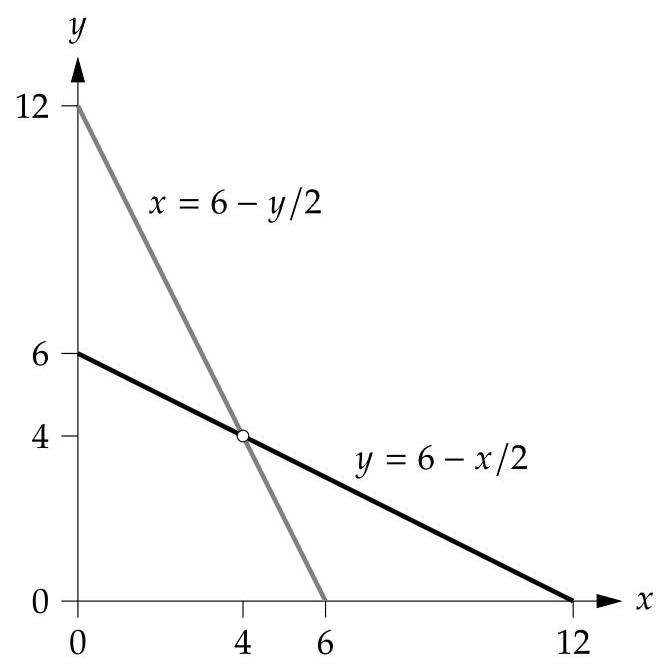
\includegraphics[width=0.4\linewidth]{translation/images/ch03-fig11.jpg}
    \caption{在双寡头博弈 \eqref{eq:3.6} 中，当\(x,y \in  \left\lbrack  {0,{12}}\right\rbrack\)时，参与人 \(\mathrm{I}\) 和参与人 II 的最优反应函数分别为\(x = 6 - y/2\) 和 \(y = 6 - x/2\)。}
    \label{fig:3.10}
\end{figure}


为了得到一个均衡 (x, y)，策略 \(x\) 和 \(y\) 必须相互为最优反应，即 \(x = 6 - y/2\) 且 \(y = 6 - x/2\)。这组线性方程有唯一解 \(x = y = 4\)，它是该博弈的唯一均衡，如图\ref{fig:3.10}中最优反应线的交点$ (4,4)$ 所示，这一均衡对应于两条最优反应曲线的交点$ (4,4)$。它与图\ref{fig:3.8}中 \(4 \times  4\) 博弈的均衡一致，其中 $4$ 恰好是所考虑的四个策略之一。

在本节余下的部分，我们将说明，即使策略集 \(\left\lbrack  {0,M}\right\rbrack\)  是无限集，也可以通过从策略集中迭代剔除整个区间内的被占优策略，使得博弈也是(近似)占优可解的。当我们选择 \(M = {12}\) 时，第一步就已经完成了:原则上，参与人 \(\mathrm{I}\) 可以选择 \({x}^{\prime } > {12}\)，但此时 \(a\left( {{x}^{\prime },y}\right)  = {x}^{\prime } \cdot  \left( {{12} - y - {x}^{\prime }}\right)  < 0\)，因为 \(y \geq  0\)，对于任何 \(y\) 来说，这都比 \(a\left( {0,y}\right)\) 更差。也就是说，如果 \({x}^{\prime } > {12}\)，那么 \({x}^{\prime }\) 被 \(x = 0\) 严格占优。同样的情况也适用于另一个参与人，所以我们可以假设两个策略集都等于区间 \(\left\lbrack  {0,{12}}\right\rbrack\)。

以下命题表明，当假设参与人 II 从区间 \(y\) 中选择策略 \(\left\lbrack  {A,B}\right\rbrack\) 时，存在另一个区间 \(\left\lbrack  {{A}^{\prime },{B}^{\prime }}\right\rbrack   = \left\lbrack  {6 - \frac{B}{2},6 - \frac{A}{2}}\right\rbrack\) 包含参与者 I 的所有可能的最优反应(条件 (a))，并且区间 \(\left\lbrack  {{A}^{\prime },{B}^{\prime }}\right\rbrack\) 之外参与者 I 的每个策略 \({x}^{\prime }\) 都被 \({B}^{\prime }\) 或 \({A}^{\prime }\) 占优(条件 (b) 和 (c))。在消除这些(被占优)策略后，我们可以假设参与者 I 仅从 \(\left\lbrack  {{A}^{\prime },{B}^{\prime }}\right\rbrack\) 中选择策略。如果两个参与者最初都在考虑来自同一区间 \(\left\lbrack  {A,B}\right\rbrack\) 的策略，那么条件 (d) 表明何时会导致一系列逐渐变窄的区间，我们将在后文对此作进一步讨论。

\begin{proposition}\label{prop:3.6}
    考虑收益由式(\ref{eq:3.6})给出的博弈，其中 \(y \in  \left\lbrack  {A,B}\right\rbrack\) 且 \(0 \leq  A \leq\)  \(B \leq  {12}\)。设 \({A}^{\prime } = 6 - \frac{B}{2}\) 且 \({B}^{\prime } = 6 - \frac{A}{2}\)。那么

(a) 区间 \(\left\lbrack  {{A}^{\prime },{B}^{\prime }}\right\rbrack\) 中的每个 \(x\) 都是参与人 \(I\)对区间 \(\left\lbrack  {A,B}\right\rbrack\) 中某个 \(y\) 的唯一最优反应。

(b) 如果 \({x}^{\prime } > {B}^{\prime }\)，那么参与人 \(I\) 的策略 \({x}^{\prime }\) 被 \(x = {B}^{\prime }\) 严格占优。

(c) 如果 \({x}^{\prime } < {A}^{\prime }\)，那么参与人 \(I\) 的策略 \({x}^{\prime }\) 被 \(x = {A}^{\prime }\) 严格占优。

(d) 区间 \(\left\lbrack  {{A}^{\prime },{B}^{\prime }}\right\rbrack\) 的长度是区间 \(\left\lbrack  {A,B}\right\rbrack\) 长度的一半，并且 \(\left\lbrack  {{A}^{\prime },{B}^{\prime }}\right\rbrack   \subseteq  \left\lbrack  {A,B}\right\rbrack\)当且仅当

\begin{equation}\label{eq:3.8}
    4 \in  \left\lbrack  {A + \frac{1}{3}\left( {B - A}\right)，A + \frac{2}{3}\left( {B - A}\right) }\right\rbrack
\end{equation}

并且如果式(\ref{eq:3.8})成立，那么用 \({A}^{\prime },{B}^{\prime }\) 代替 \(A,B\) 时它也成立。

\end{proposition}

\begin{figure}
    \centering
    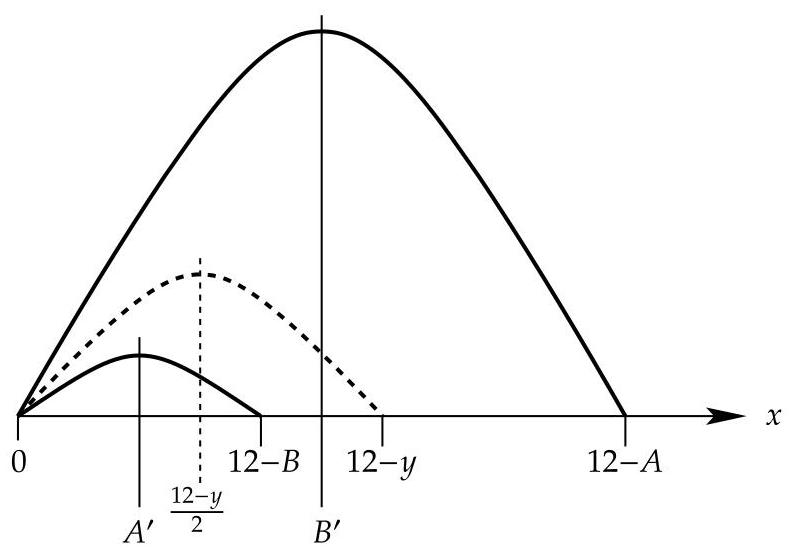
\includegraphics[width=0.5\linewidth]{translation/images/ch03-fig12.jpg}
    \caption{虚线曲线展示了命题~\ref{prop:3.6}中参与人I的收益 \(x \cdot  \left( {{12} - y - x}\right)\) (负收益未显示)。其最大值位于 \(\frac{{12} - y}{2}\) 处。这里 \({A}^{\prime } = \frac{{12} - B}{2}\) 和 \({B}^{\prime } = \frac{{12} - A}{2}\)}
    \label{fig:3.11}
\end{figure}


证明。假设参与人II在 \(\left\lbrack  {A,B}\right\rbrack\) 中选择某个 \(y\)。根据式(\ref{eq:3.7})，参与人I的收益作为 \(x\) 的函数是一条抛物线。图\ref{fig:3.11}展示了两种极端情况\(y = A\) 和 \(y = B\) (实线曲线)以及一个中间情况(虚线曲线)。参与人 I 对 \(y\) 的最优反应是 \(x = \frac{{12} - y}{2}\)，在 \(\frac{{12} - B}{2}\) 和 \(\frac{{12} - A}{2}\) 之间，即在区间 \(\left\lbrack  {{A}^{\prime },{B}^{\prime }}\right\rbrack\) 内，如图 \ref{fig:3.11} 中的长实线垂直线所示。映射 \(\left\lbrack  {A,B}\right\rbrack   \rightarrow  \left\lbrack  {6 - \frac{B}{2},6 - \frac{A}{2}}\right\rbrack ，y \mapsto  6 - \frac{y}{2}\) 是一个双射，这表明了条件 (a)。

情况 \(y = A\) 对参与人I来说是最有利的，这对应图\ref{fig:3.11}中最高的抛物线。该图表明，如果 \({x}^{\prime } > {B}^{\prime } = \frac{{12} - A}{2}\)，那么参与者 \(\mathrm{I}\) 选择 \(x = {B}^{\prime }\) 肯定更有利，因为对于每个 \(y \geq  A\)，虚线抛物线从 \({B}^{\prime }\) 到 \({x}^{\prime }\) 是向下倾斜的(甚至可能取负值)。下面对条件 (b) 进行严格证明。设 \({x}^{\prime } > {B}^{\prime }\)。我们要证明 \(a\left( {{B}^{\prime },y}\right)  > a\left( {{x}^{\prime },y}\right)\)，根据式(\ref{eq:3.7})，这等价于

\begin{equation}\label{eq:3.9}
    -{\left( {B}^{\prime } - \frac{{12} - y}{2}\right) }^{2} >  - {\left( {x}^{\prime } - \frac{{12} - y}{2}\right) }^{2}\text{ . } 
\end{equation}
结合

\[
{x}^{\prime } = {B}^{\prime } + c\;\left( {c > 0}\right)，\;y = A + d\;\left( {d \geq  0}\right)
\]
因此 \(\frac{{12} - y}{2} = 6 - \frac{A + d}{2} = {B}^{\prime } - \frac{d}{2}\)，不等式\ref{eq:3.9}等价于

\[
{\left( {B}^{\prime } - \left( {B}^{\prime } - \frac{d}{2}\right) \right) }^{2} < {\left( {B}^{\prime } + c - \left( {B}^{\prime } - \frac{d}{2}\right) \right) }^{2},
\]
即 \({\left( d/2\right) }^{2} < {\left( c + d/2\right) }^{2}\)，这是成立的。这证明了(b)。

类似地，情况 \(y = B\) 对参与者 \(\mathrm{I}\) 来说是最不利的，这对应图\ref{fig:3.11}中最低的抛物线。那么如果 \({x}^{\prime } < {A}^{\prime } = \frac{{12} - B}{2}\)，参与者I选择 \(x = {A}^{\prime }\) 更有利，因为对于每个 \(y \leq  B\)，抛物线从 \({x}^{\prime }\) 到 \({A}^{\prime }\) 是向上倾斜的。正式地，设 \({x}^{\prime } < {A}^{\prime }\)。我们要证明 \(a\left( {{A}^{\prime },y}\right)  > a\left( {{x}^{\prime },y}\right)\)，即
\begin{equation}\label{eq:3.10}
   - {\left( {A}^{\prime } - \frac{{12} - y}{2}\right) }^{2} >  - {\left( {x}^{\prime } - \frac{{12} - y}{2}\right) }^{2}\text{ . }  
\end{equation}
现在我们设

\[
{x}^{\prime } = {A}^{\prime } - c\;\left( {c > 0}\right)，\;y = B - d\;\left( {d \geq  0}\right)
\]
因此 \(\frac{{12} - y}{2} = 6 - \frac{B - d}{2} = {A}^{\prime } + \frac{d}{2}\)。那么式\ref{eq:3.10}等价于
\[
{\left( {A}^{\prime } - \left( {A}^{\prime } + \frac{d}{2}\right) \right) }^{2} < {\left( {A}^{\prime } - c - \left( {A}^{\prime } + \frac{d}{2}\right) \right) }^{2},
\]

即 \({\left( -d/2\right) }^{2} < {\left( -c - d/2\right) }^{2}\) 或者再次得到 \({\left( d/2\right) }^{2} < {\left( c + d/2\right) }^{2}\)，这是成立的。这证明了(c)。

为了证明(d)，显然 \({B}^{\prime } - {A}^{\prime } = \left( {B - A}\right) /2\)。条件 \(\left\lbrack  {{A}^{\prime },{B}^{\prime }}\right\rbrack   \subseteq  \left\lbrack  {A,B}\right\rbrack\) 等价于 \(A \leq  {A}^{\prime } = 6 - \frac{B}{2}\) 和 \({B}^{\prime } = 6 - \frac{A}{2} \leq  B\)，它有以下等价表述:

\[
A + \frac{B}{2} \leq  6 \leq  B + \frac{A}{2},
\]

\[
A + \frac{A + \left( {B - A}\right) }{2} \leq  6 \leq  A + \left( {B - A}\right)  + \frac{A}{2},
\]

\[
\frac{3}{2}A + \frac{\left( B - A\right) }{2} \leq  6 \leq  \frac{3}{2}A + \left( {B - A}\right)，
\]

即
\begin{equation}\label{eq:3.11}
    A + \frac{1}{3}\left( {B - A}\right)  \leq  4 \leq  A + \frac{2}{3}\left( {B - A}\right)
\end{equation}

这在(\ref{eq:3.8})中有所陈述。假设\ref{eq:3.11}成立，我们想证明用 \({A}^{\prime },{B}^{\prime }\) 代替 \(A,B\) 时的相同不等式，即
\[
{A}^{\prime } + \frac{1}{3}\left( {{B}^{\prime } - {A}^{\prime }}\right)  \leq  4 \leq  {A}^{\prime } + \frac{2}{3}\left( {{B}^{\prime } - {A}^{\prime }}\right)，
\]

\[
{B}^{\prime } - \frac{2}{3}\left( {{B}^{\prime } - {A}^{\prime }}\right)  \leq  4 \leq  {B}^{\prime } - \frac{1}{3}\left( {{B}^{\prime } - {A}^{\prime }}\right)，
\]

\[
6 - \frac{A}{2} - \frac{2}{3}\left( {{B}^{\prime } - {A}^{\prime }}\right)  \leq  4 \leq  6 - \frac{A}{2} - \frac{1}{3}\left( {{B}^{\prime } - {A}^{\prime }}\right)
\]
或者

\[
2 \leq  \frac{A}{2} + \frac{2}{3}\left( {{B}^{\prime } - {A}^{\prime }}\right)，\;\frac{A}{2} + \frac{1}{3}\left( {{B}^{\prime } - {A}^{\prime }}\right)  \leq  2
\]

将其乘以$ 2$ 并结合 \(2\left( {{B}^{\prime } - {A}^{\prime }}\right)  = B - A\) 后，等价于我们假设为真，因此所需结论成立，完成了条件(d)的证明。

根据命题\ref{prop:3.6}，我们可以对博弈\ref{fig:3.6}应用重复剔除被占优策略，具体如下。假设两个参与人都可以选择区间 \(\left\lbrack  {A,B}\right\rbrack   = \left\lbrack  {0,{12}}\right\rbrack\) 内的任何策略。可以得到 \(\left\lbrack  {{A}^{\prime },{B}^{\prime }}\right\rbrack   = \left\lbrack  {0,6}\right\rbrack\)。参与人 I 在 \(\left\lbrack  {{A}^{\prime },{B}^{\prime }}\right\rbrack\) 之外的任何策略 \({x}^{\prime }\) (这里仅指 \({x}^{\prime } > 6\) )都被 \(x = {B}^{\prime }\) 占优。(然而，如(a)中所述， \(\left\lbrack  {{A}^{\prime },{B}^{\prime }}\right\rbrack\) 内的任何策略都不被占优，因为它是对 \(\left\lbrack  {A,B}\right\rbrack\) 中某个 \(y\) 的最优反应，这表明此阶段的剔除是最优的。)类似地，由于该博弈是对称的，参与人 II 在 \(\left\lbrack  {{A}^{\prime },{B}^{\prime }}\right\rbrack\) 之外的任何策略 \({y}^{\prime }\) 都被 \(y = {B}^{\prime }\) 占优。我们剔除这些被占优策略，使得新的策略集将是 \(\left\lbrack  {{A}^{\prime },{B}^{\prime }}\right\rbrack\)。条件(\ref{eq:3.8})表明 4 在区间 \(\left\lbrack  {A,B}\right\rbrack\) 的中间三分之一处，如果 \(\left\lbrack  {A,B}\right\rbrack   = \left\lbrack  {0,{12}}\right\rbrack\) 成立，这一条件恰好成立，其中中间三分之一是 \(\left\lbrack  {4,8}\right\rbrack\)。此外，条件(d)表明对于 \(\left\lbrack  {{A}^{\prime },{B}^{\prime }}\right\rbrack\) 同样成立(实际上，4 在区间 \(\left\lbrack  {0,6}\right\rbrack\) 的中间三分之一 \(\left\lbrack  {2,4}\right\rbrack\) 处)。我们现在可以用 \({A}^{\prime },{B}^{\prime }\) 代替 \(A,B\) 重复剔被占优策略，并且每次所考虑区间的长度 \(B - A\) 都会减半。策略 \(x = 4\) 和 \(y = 4\) 属于所有这些区间。实际上，除$(4,4)$外任何其他策略迟早都会处于足够小的区间之外，因此会被剔除。不过，对于非常接近 \(4\) 的策略，需要经过多少轮剔除并不存在统一的上界。最终，只有策略组合(4,4)留存下来，这是该博弈的唯一均衡。

这表明数量竞争的双寡头博弈\ref{fig:3.6}是占优可解的，如果允许进行无限多轮剔除，就可以得到这一结论；如果只允许有限轮剔除，则可以达到任意给定的精度。占优可解性被认为是比均衡更强的解概念。当然，该博弈的均衡本身也可以直接求得，即联立方程 \(x = 6 - y/2\) 和 \(y = 6 - x/2\)。

\section{没有纯策略均衡的博弈}

并非每个博弈都存在纯策略均衡。图~\ref{fig:3.12}展示了两个著名的例子。在硬币匹配中，两名参与者各出示一枚硬币，硬币可能正面(H)朝上或反面(T)朝上。如果两枚硬币的正反面相同，则参与人I赢得对方的硬币；否则，参与人II赢得硬币。任何策略组合都不可能是稳定的，因为处于劣势的一方总是有激励改变自己的策略。

\begin{figure}
    \centering
    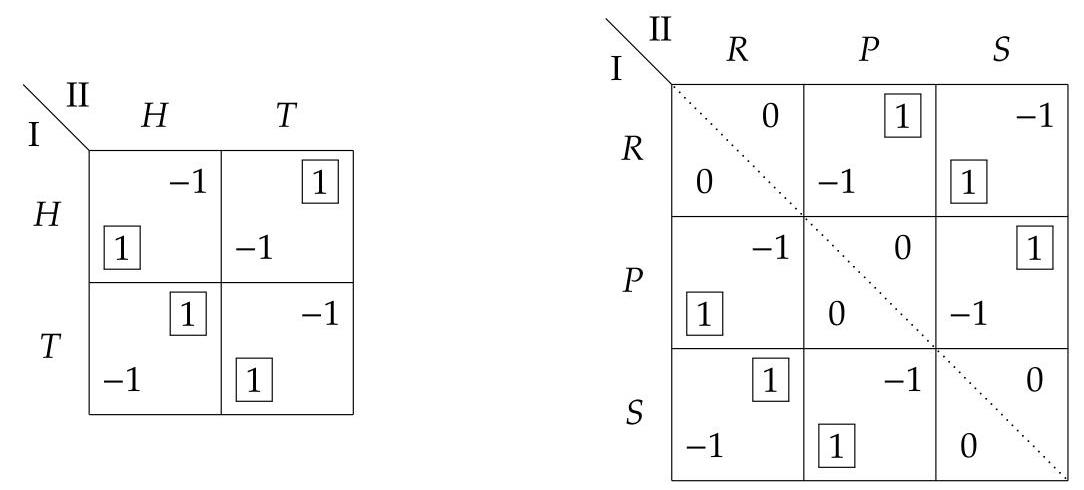
\includegraphics[width=0.7\linewidth]{translation/images/ch03-fig13.jpg}
    \caption{硬币匹配(左)和石头剪刀布(右)。}
    \label{fig:3.12}
\end{figure}

石头剪刀布是一个 \(3\times3\) 博弈，两名参与者同时从石头(R)、布(P)、剪刀(S)这三种策略中选择其一。石头输给布，布输给剪刀，剪刀输给石头；若双方选择相同，则为平局。不存在互为最优反应的策略组合。与硬币匹配一样，石头剪刀布也是一个零和博弈，因为收益表中任意单元格内双方的收益之和均为零。与硬币匹配博弈不同的是，石头剪刀布是一个对称博弈。因此，当两名参与人选择相同的策略时(即收益表对角线上的单元格)，双方获得相同的收益；又由于该博弈是零和博弈，因此此时双方的收益均为零。

对于硬币匹配或石头剪刀布这类不存在纯策略均衡的博弈，博弈论给出的建议是按照由收益决定的特定概率随机选择策略。正如我们将在第6章中看到的，当允许参与人采用随机化策略时，任何有限博弈都存在均衡。

\section{每个参与人有两种策略的对称博弈}

在本节中，我们考虑一类 \(N\) 人博弈：每个参与人只有两种策略，并且博弈是对称的。令人惊讶的是，这类博弈总是存在纯策略均衡。

如果每个参与人都具有相同的策略集，并且对参与人进行任意置换、同时相应地置换其收益后，博弈仍然保持不变，那么这个 \(N\) 人博弈就是对称的。对于两人博弈而言，这意味着交换两个参与人及其相应的收益后，博弈保持不变。在收益矩阵中，这可以直观地表示为沿对角线进行反射。

现在我们考虑对称的n人博弈，其中每个参与人有两种策略，我们称之为0和1。通常，这些策略的任何组合都定义了一个单独的策略组合，因此有$2^N$个组合，并且每个组合都为每个参与人指定了一个收益，所以该博弈由$N \cdot 2^N$个收益来定义。如果该博弈是对称的，则需要的收益数量会大大减少。此时，一个策略组合由选择1的参与人数量决定，假设为$k$名参与人选择1(其中0 ≤ k ≤ n)，然后剩下的$n - k$名参与人选择0，该策略组合可以写成

\begin{equation}\label{eq:3.12}
    \left( {\underset{k}{\underbrace{1,\ldots，1}},\underset{N - k}{\underbrace{0,\ldots，0}}}\right) .
\end{equation}

由于该博弈是对称的，只要有 \(k\) 名参与人选择策略1，那么任何这样的策略组合中，所有选择策略1的参与人获得的收益都必须与式\ref{eq:3.12}中选择策略1的参与人的收益相同；同样，所有选择策略0的参与人也获得另一个相同的收益。因此，当$1 \leq k \leq N-1$时，对于式\ref{eq:3.12}所表示的这类策略组合，只需要两个收益。当$k = 0$时，策略组合为$(0, \ldots, 0)$，所有参与人都选择相同的策略0，因此只需要一个收益；类似地，当$k = N$时，所有参与人都选择策略1，也只需要一个收益。因此，每个参与人有两种策略的对称 \(N\) 人博弈只需要由$2N$个收益来描述。

\begin{proposition}\label{prop:3.7}
    考虑一个对称的n人博弈，其中每个参与人有两种策略，0和1。那么这个博弈存在纯策略均衡。当且仅当策略1占优于策略0时，策略组合$(1, \ldots, 1)$是该博弈的唯一均衡。
\end{proposition}

\begin{proof}
如果策略1占优策略0，那么 \((1,1,\ldots,1)\) 显然是该博弈的唯一均衡。下面假设策略1不占优策略0。由于每个参与人只有策略0和1两种选择，因此必定存在其他参与人的某个策略组合，使得选择策略0所获得的收益大于或等于选择策略1所获得的收益；也就是说，在这种情况下，策略0是一个最优反应。

考虑一个形如\ref{eq:3.12}的策略组合，其中策略0是一个最优反应，并在所有这样的策略组合中选择使得采用策略1的参与人人数 \(k\) 最少的一个，其中 \(0\leq k<N\)。我们证明这个策略组合是一个均衡。

根据假设和博弈的对称性，对于每个选择策略0的参与人而言，策略0都是对其他参与人策略的最优反应。现在考虑选择策略1的参与人。如果其中某个参与人的策略1不是最优反应，那么由于该参与人只有两个策略，他将通过把策略从1改为0而获得更高的收益。这样便得到一个新的策略组合，其中只有 \(k-1\) 名参与人选择策略1，而且对于刚刚改变策略的参与人而言，策略0是一个最优反应。由对称性，在这一新的策略组合中，策略0是选择策略0的参与人的最优反应。这与 \(k\) 的最小性相矛盾。

因此，每个选择策略1的参与人也都在采取最优反应。于是该策略组合中的每个参与人都在采取对其他参与人策略的最优反应，因此它是一个纯策略均衡。
\end{proof}


下面考虑命题\ref{prop:3.7}在\(N = 2\)时的情形。对称的囚徒困境博弈(图\ref{fig:3.1})只有一个均衡，并且该均衡确实采用了占优策略。这个均衡是对称的，即两个参与人选择相同的策略。对称的猎鹿博弈(图\ref{fig:3.5})有两个对称均衡。对称的胆小鬼博弈(图\ref{fig:3.3})则有两个非对称均衡。显然，在任何对称的两人博弈中，非对称均衡总是成对出现。例如，这里的两个均衡为 \((A,C)\) 和 \((C,A)\)，二者可以通过交换两个参与人及其策略得到。胆小鬼博弈不存在对称的纯策略均衡。 \(3 \times 3\) 的石头剪刀布博弈(图\ref{fig:3.12})也是对称的，但它不存在纯策略均衡。这说明命题\ref{prop:3.7}不能推广到每个参与人拥有两种以上策略的对称博弈。
\begin{center}
\setlength{\fboxsep}{6pt}
\setlength{\fboxrule}{0.4pt}
\fbox{
    \parbox{\dimexpr\linewidth-2\fboxsep-2\fboxrule\relax}{
        \ \(\Rightarrow\) 练习~\ref{exer:3.4} 描述了一个与命题~\ref{prop:3.7} 相关的博弈。
    }
}
\end{center}

\section{延伸阅读}

收益表中每个单元格的两个收益分别错位排列在左下角和右上角，这种表示方式源于托马斯·谢林(Thomas Schelling)。2005年，他与罗伯特·奥曼(Robert Aumann)共同获得诺贝尔经济学奖(正式名称为“瑞典中央银行纪念阿尔弗雷德·诺贝尔经济学奖”)，获奖理由是“通过博弈论分析增进了我们对冲突与合作的理解”。根据迪克西特(Dixit)和奈尔伯夫(Nalebuff)(1991年，第90页)的记载，谢林曾十分谦逊地说：“如果有人问我是否曾对博弈论作出过贡献，我会回答‘是的’；如果再问我的贡献是什么，我会说，是发明了矩阵中这种错位排列收益的方式。”

策略式是每门非合作博弈论课程都会讲授的内容(它有时也被称为“标准式”，但如今这一称呼在博弈论中使用得较少，因为“标准”一词在数学中已经被广泛用于许多不同的含义)。Osborne (2004)对本章讨论的各种博弈及其历史背景作了细致介绍，其中包括Cournot (1838)最初提出的双寡头模型，以及许多其他博弈。本书的练习~\ref{exer:3.4} 取自该书。Gibbons(1992)证明了古诺博弈是占优可解的，不过其论证不如我们对命题~\ref{prop:3.6} 的证明详细。Osborne和Gibbons都没有采用谢林提出的这种收益表示方式，而是像定义~\ref{def:3.1} 中那样，使用以逗号分隔的收益。

3.6节中的古诺博弈同时也是一个势博弈，其势函数严格凹，因此具有唯一的最大值，从而该博弈具有唯一均衡。Neyman(1997)进一步证明，该均衡也是该博弈唯一的相关均衡(见第12章)。Monderer and Shapley(1996)提出的势博弈将具有势函数的博弈推广为更一般的一类博弈，其中包括2.5节讨论的拥塞博弈。

关于均衡精炼的经典综述可参见van Damme (1987)。命题\ref{prop:3.7}似乎最早由Cheng、Reeves、Vorobeychik和Wellman(2004年，定理1)证明。

\section{第3章练习}

\begin{exercise}\label{exer:3.1}
考虑以下 \(3\times3\) 博弈。

\begin{center}
    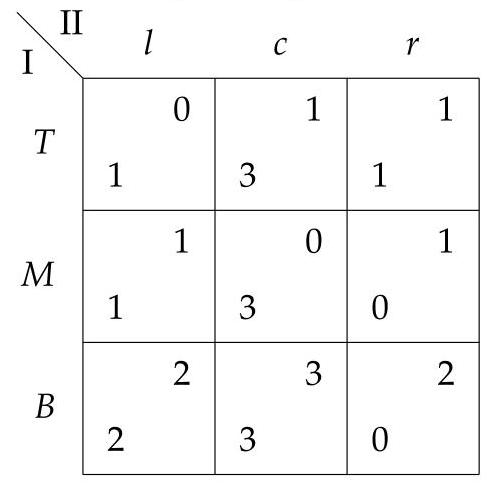
\includegraphics[width=0.38\linewidth]{translation/images/ch03-fig14.jpg}
\end{center}

\begin{enumerate}
\renewcommand{\labelenumi}{(\alph{enumi})}
\setlength{\itemsep}{0.4em}

\item 找出所有策略对，其中一个策略弱占优另一个策略。

\item 假设允许你剔除某个参与人的一个弱被占优策略。进行此操作，并重复这一过程（即迭代剔除弱被占优策略），直到得到原博弈的一个单一策略组合。（注意：两个收益等价的策略并不相互弱占优！）

\item 找出另一种迭代剔除弱被占优策略的方式，使其最终得到一个不同于(b)中结果的策略组合，并且两个策略以及参与人的收益均与(b)中的结果不同。

\item 该博弈的（纯策略）均衡是什么？

\end{enumerate}
\end{exercise}


\begin{exercise}\label{exer:3.2}
考虑以下策略式的三人博弈。

\begin{center}
\begin{minipage}[t]{0.40\linewidth}
    \centering
    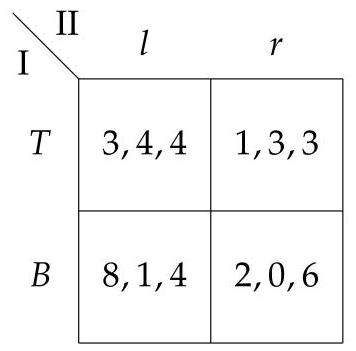
\includegraphics[width=0.8\linewidth]{translation/images/ch03-fig15.jpg}

    \vspace{0.2em}
    III: \(L\)
\end{minipage}
\hspace{0.06\linewidth}
\begin{minipage}[t]{0.40\linewidth}
    \centering
    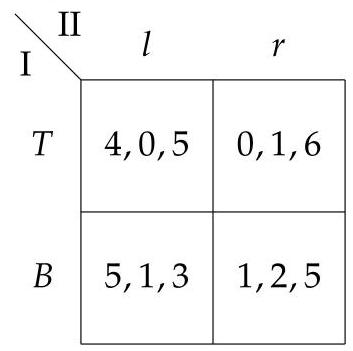
\includegraphics[width=0.8\linewidth]{translation/images/ch03-fig16.jpg}

    \vspace{0.2em}
    III: \(R\)
\end{minipage}
\end{center}

每个参与人都有两种策略：参与人 I 的策略为 \(T\) 和 \(B\)（分别对应上行和下行）；参与人 II 的策略为 \(l\) 和 \(r\)（分别对应每个 \(2\times2\) 面板中的左列和右列）；参与人 III 的策略为 \(L\) 和 \(R\)（分别对应左面板和右面板）。每个单元格中的收益均以三元组的形式给出，并依次对应参与人 I、II 和 III 的收益。

\begin{enumerate}
\renewcommand{\labelenumi}{(\alph{enumi})}
\setlength{\itemsep}{0.4em}

\item 找出所有满足一个策略严格占优或弱占优另一个策略的策略对。\textit{[提示：确保你理解在两个以上参与人的博弈中占优的含义，并注意比较正确的收益。]}

\item 对该博弈进行迭代剔除严格被占优策略。该博弈的均衡是什么？

\end{enumerate}
\end{exercise}


\begin{exercise}\label{exer:3.3}
考虑第3.6节研究的双寡头博弈，其中参与人 I 和 II 分别选择非负产量 \(x\) 和 \(y\)，市场上的单位价格为 \(12-x-y\)。现在进一步考虑生产成本：参与人 I 的单位生产成本为1，参与人 II 的单位生产成本为2。写出式\eqref{eq:3.6}相应的收益函数，求出两个参与人的最优反应函数，并确定该博弈的均衡。均衡时两个参与人的利润分别是多少？
\end{exercise}


\begin{exercise}\label{exer:3.4}
(Osborne, 2004, Exercise 33.1, \textit{Contributing to a public good}.)

\(N\) 个人中的每个人都选择是否为公共品的提供贡献一笔固定金额。当且仅当至少有 \(K\) 个人做出贡献时，该公共品才会被提供，其中 \(2\leq K\leq N\)。如果公共品最终未被提供，已经做出的贡献也不会退还。每个人对各种结果的严格偏好由高到低排列如下：

\begin{enumerate}
\renewcommand{\labelenumi}{(\roman{enumi})}
\setlength{\itemsep}{0.2em}

\item 公共品被提供，并且她没有做出贡献；

\item 公共品被提供，并且她做出了贡献；

\item 公共品未被提供，并且她没有做出贡献；

\item 公共品未被提供，并且她做出了贡献。

\end{enumerate}

将上述情形表示为一个策略式博弈，并找出其均衡。你需要明确参与人的数量、每个参与人可选择的策略，以及参与人对不同策略组合的偏好。这个博弈具有对称性吗？是否存在超过 \(K\) 个人做出贡献的均衡？是否存在恰好 \(K\) 个人做出贡献的均衡？是否存在少于 \(K\) 个人做出贡献的均衡？
\end{exercise}
